\documentclass[11pt,a4paper]{article}
\usepackage[top=1.0in,bottom=1.0in,left=1.0in,right=1.0in]{geometry}

\usepackage{xurl}
\usepackage{graphicx}
\usepackage{float}

\usepackage{csquotes}
\usepackage[natbib=true,
            style=ieee,
            sorting=none,
            citestyle=numeric-comp
            ]{biblatex}
\addbibresource{bibliography.bib}
\usepackage{hyperref}

\title{Kernel Density Estimates for Quantifying Material Domains}

\usepackage{authblk}
\author[a]{Lane E. Schultz}
\author[d]{Yiqi Wang}
\author[a]{Doyeon Kim}
\author[a]{Ryan Jacobs}
\author[a]{Dane Morgan}
\author[b,c]{Aristana Scourtas}
\author[b,c]{K.J. Schmidt}
\author[b,c]{Ben Blaiszik}

\affil[a]{University of Wisconsin-Madison, 1500 engineering Drive, Madison, WI 53706, USA}
\affil[b]{Argonne National Laboratory, Data Science and Learning Division, Chicago, Lemont 60439, USA}
\affil[c]{University of Chicago, Globus, Chicago 60637, USA}
\affil[d]{Carnegie Mellon University, 5000 Forbes Ave, Pittsburgh, PA 15213, USA}

\date{\today}

\begin{document}

\maketitle

\section{Target Journals}

\begin{enumerate}
    \item Computational Material Science (Elsevier)
    \item NPJ Computational Materials
    \item Nature Computational Science
    \item Journal of Material Informatics (OAE)
\end{enumerate}

\section{Key Goals}

\begin{itemize}
    \item Demonstrate the use of kernel density estimates (KDE) for quantifying material domains via three methods:
    \begin{enumerate}
        \item A chemical intuition method that involves grouping materials based on their chemical constituents, which relies on a researcher's knowledge of chemistry to discern domains.
        \item A single valued numerical approach which studies the residual from predictions on split data with repeated cross fold validation and a bootstrapped leave one cluster out. The single valued approach is applicable to a wider range of model types compared to methods that rely on models capable of providing uncertainty estimates. This is because the single valued approach does not depend on the availability of uncertainty estimation capabilities within the models.
        \item A statistical numerical approach where sampled z-scores are compared to standard normal distributions for binned data. In contrast to the single value numerical approach, our statistical method examines both uncertainty estimates and residuals to assess situations where uncertainty measures inadequately reflect actual model errors.
    \end{enumerate}
    \item While method 1 relies on a researcher's intuition regarding the chemical domain, methods 2 and 3 are more general and do not require such domain-specific knowledge. For methods 2 and 3 to have a chance of success, it is crucial for method 1 to be effective. The success of method 1 sets the stage and provides a necessary foundation for the subsequent methods to yield meaningful results.
    \item The numerical approaches use KDE to build models that can predict in-domain (ID) and out-of-domain (OD) samples.
\end{itemize}

%\begin{abstract}
    fill in later
\end{abstract}

{\bf Keywords:} Chemistry, Machine learning, Domain, Uncertainty Quantification
\section{Variables, Definitions, and Acronyms}

\begin{itemize}
    \item $y$: The target variable for regression
    \item $\hat{y}$: The predicted target variable
    \item $\sigma_{y}$: The standard deviation of the target variable used for fitting a model
    \item $\sigma_{u}$: The uncalibrated uncertainty from ensemble models
    \item $\sigma_{c}$: The calibrated uncertainty from ensemble models
    \item $z$: $z=\frac{y-\hat{y}}{\sigma_{c}}$ and is also called the z-score
    \item $T_{high}$: $T_{C}$ $>$ 50 $[K]$
    \item $T_{low}$: $T_{C}$ $\leq$ 50 $[K]$
    \item MAE: Mean Average Error
    \item RMSE: Root Mean Squared Error
    \item $R^{2}$: The coefficient of determination
    \item PR: Precision Recall
    \item PR Baseline: The number of positive classes over the number of total classes
    \item AUC: Area under the Curve
    \item Relative AUC: The fraction of total area above the PR Baseline that a PR curve covers
    \item UQ: Uncertainty Quantification
    \item KDE: Kernel Density Estimate
    \item D: The dissimilarity metric of choice (may use 1-KDE, D, and dissimilarity interchangeably but need to agree on a convention. I like D personally.)
    \item PPB: Points Per Bin
    \item CV: Cross Validation
    \item ID: In Domain
    \item OD: Out of Domain
    \item PDF: Probability Density Function
    \item CDF: Cumulative Distribution Function
    \item Miscalibration Area: The area between an observed CDF and a standard normal CDF
    \item MAST-ML: Materials Simulation Toolkit for Machine Learning
    \item MSE: Materials Science and Engineering
\end{itemize}
\section{Introduction}

\begin{enumerate}

    \item While machine learning has made remarkable advances in numerous fields, it is crucial to exercise caution when applying a model. Although models often exhibit impressive performance on test data that is sampled similarly to the training data, they can experience performance degradation when deployed in real-world scenarios.
    
    \item Discuss current research on changes/shifts in domains and their impact on model reliability. Many examples are included in \cite{Koh2020}.

    \item When developing a machine learning (ML) model, three key factors contribute to its overall effectiveness:

    \begin{enumerate}
        \item Accuracy: This refers to the model's ability to make precise and accurate predictions. Achieving high accuracy is a fundamental goal in supervised ML studies.
        \item Precision: In addition to accuracy, precision involves ensuring that the model's error bars or uncertainty estimates are reliable and accurately reflect the level of uncertainty associated with the predictions.
        \item Applicability: Applicability refers to the ability of the model to provide reliable predictions within its intended domain. It is crucial that the model's predictions are applicable and valid within the specific context for which it was trained. This aspect ensures that the model's outputs are meaningful and reliable for the intended use case.
    \end{enumerate}

    \item While a significant amount of ML research in the materials science and engineering (MSE) focuses on achieving accuracy (point 1), there has been increasing attention towards precision (point 2) in recent years. However, relatively less emphasis has been placed on addressing applicability (point 3), which remains an area with significant untapped potential.

    \item Our research addresses the crucial aspect of applicability (point 3) while also providing a comprehensive framework that encompasses accuracy, precision, and applicability. By tackling all three aspects, our research contributes to a more comprehensive and robust approach in ML studies within the MSE field.
    
    \item A first step in determining whether a prediction is reliable is through uncertainty quantification. Uncertainty quantification has been extensively studied in both classification and regression settings to assess the reliability of predictions and have many well-developed techniques \cite{Abdar2021, Scalia2020, Tran2019, Caruana2005, Kull2017}. Often, there is a need to enhance the reliability of uncertainty measures by introducing modifications to make them more robust and dependable.
    
    \begin{enumerate}
    
        \item Define calibration: ``Calibration of a model refers to the property of outputting probability distributions that are consistent with observed empirical frequencies'' \cite{Scalia2020}.
        
        \begin{enumerate}
            \item Classification: Platt scaling or isotonic regression \cite{Caruana2005}.
            \item Regression: Parametric models or isotonic regression \cite{Busk2022, Morgan2020, Hirschfeld2020}.
        \end{enumerate}
        
        \item Mention the many ways one can assess whether uncertainties are calibrated \cite{Pernot2022}.
        
        \item Discuss non-deep ensemble models as seen in Glen Palmer's work \cite{Palmer2022}.
        
    \end{enumerate}
    
\item The reliability of uncertainty predictions, even when calibrated, is limited to the model's domain of applicability. This limitation can be likened to a pendulum problem, where the model's uncertainty quantification tends to deteriorate when making predictions on data with features outside the range of what the model was trained on \cite{Caldeira2020}. In the supplemental section of the research paper by Palmer et al. (2022), additional work demonstrates that uncertainties lose their reliability when applied beyond the chemical domain of a model \cite{Palmer2022}.

\item It is crucial to conduct a thorough analysis of the model's underlying data space to prevent its application on significantly dissimilar data. By studying the boundaries and characteristics of the data space, we can effectively identify instances where caution is necessary before applying the model.

\item Comparing the space of training data and a test sample is an intuitive concept to study domain. Model-agnostic spatial approaches include convex hulls, distance measures, probability density estimates, et cetera \cite{Jaworska2005}. Additionally, researchers have achieved promising results by studying the latent space of neural networks. Studies have revealed that test samples closer in the training latent space tend to exhibit lower errors compared to those farther away, as demonstrated by Janet et al. \cite{Janet2019}. In the machine learning field of domain adaptation, researchers aim to enhance a model's performance and generalization capabilities by modifying either the test data or model parameters with respect to differences between training and testing space \cite{domain_adaptation, de2021adapt}.

\item Our research focuses on evaluating the effectiveness of probability density estimates using Kernel Density Estimation (KDE) as a means to distinguish domains. We employ three distinct approaches: chemical intuition, single numerical techniques, and statistical numerical techniques. For relevant data sets, we generate features for materials with known target variables, as well as materials with unknown target variables in other chemical groups and measure KDE. Our findings demonstrate that KDE can effectively separate chemical groups, aligning with chemical intuition.

\item On the numerical front, we illustrate that individual predictions for data located further away from the training data exhibit higher residuals overall. We propose a residual cutoff as a means to identify both ID and OD data. Furthermore, we compare the statistics from subsets of all predictions with an expected distributions. Our results reveal that data located further away from the training data deviate from the expected patterns.
\end{enumerate}
\section{Methods}

\subsection{Software Tools Used}
\begin{itemize}
    \item Machine Learning and Feature Generation: Materials Simulation Toolkit for Machine Learning (MAST-ML) \cite{Jacobs2020}.
    \item Machine Learning: Scikit-learn \cite{scikit-learn}.
    \item Text Refinement: ChatGPT \cite{gpt-3.5}.
\end{itemize}

\subsection{Definition of Techniques}

\begin{enumerate}

    \item General Method for Uncertainty Quantification:

    \begin{enumerate}
        \item Start with an ensemble model (random forest regressor).
        \item Acquire individual predictions from each model from the ensemble.
        \item Calculate standard deviation of predictions, $\sigma_{u}$.
        \item Calibrate uncertainties by minimizing log likelihood function as shown in \cite{Palmer2022}.
        \item Our new, calibrated uncertainties become $\sigma_{c}=a\sigma_{u}+b$, where $a$ and $b$ are constants.
    \end{enumerate}

    \item General Method for KDE:

    \begin{enumerate}
        \item Features are standardized using standard scaler fit from training data.
        \item A single bandwidth parameter is used with Gaussian kernels. The bandwidth is estimated automatically using a nearest neighbors algorithm as implemented in Scikit-learn. Specifically, we use the sklearn.cluster.estimate\_bandwidth method \cite{scikit-learn}.
        \item Likelihoods are acquired from training data, and are shifted so that the maximum likelihood case is 1 because values are often very small otherwise.
        \item We then transform scores by: 1-score which we call D.
        \item When a KDE model is used to predict on cases, the likelihood is computed, shifted by the maximum likelihood value from training, and then transformed by 1-score.
        \item Values of 1 means the point is not observed, and decreasing values are more likely to be observed.
    \end{enumerate}

    \item General Method for Chemical Domain Tests. For observation i from the original set of data containing the target variable:

        \begin{enumerate}
            \item Leave out sample i from the original set, and leave out all other cases that do not have target variables.
            \item Train a regression model on the left in data and calibrate uncertainties.
            \item Fit a KDE with a Gaussian kernel on the left in data.
            \item Predict $\hat{y}$, $\sigma_{c}$, and $D$ on the left out data.
            \item We repeat the procedure for all cases in the original set and aggregate data. If there are $n$ cases that contain target variables, then there should be $n$ different models by the time the procedure finishes.
        \end{enumerate}

    \item General Method for Single Numerical Tests:

    \begin{enumerate}
        \item Start with any subset of data that contains target variables.
        
        \item Split the data for 5-fold cross validation (CV). Iteratively fit on 4 folds and then predict $\hat{y}$, $\sigma_{c}$, and $D$ on left out data of 1 fold.
        
        \item Pre-cluster data using agglomerate clustering. Iteratively bootstrap samples from all clusters, leave one cluster out for testing, and use all other clusters to train model. Then, predict $\hat{y}$, $\sigma_{c}$, and $D$ on the left out data. Perform clustering to produce 2 and 3 clusters, which is similarly applied in \cite{loco, Meredig2018}. We can repeatedly perform this procedure with slightly different data for each model due to boostrapping.
        
        \item Aggregate all statistics on left out data.
        
        \item Calculate $\sigma_{y}$, normalize absolute residuals by $\sigma_{y}$ ($|y-\hat{y}|/\sigma_{y}$) for each test case, and define ID as cases that score less than 1 of $|y-\hat{y}|/\sigma_{y}$ (OD otherwise). Below a value of 1, we can yield predictions that have an error less than $\sigma_{y}$, which serves as a measure of data dispersion. Our objective is to keep predictions with residuals smaller in magnitude than the dispersion of the data. By doing so, we aim to ensure that the model's predictions are statistically significant and meaningful relative to the inherent variability present in the data.
        
        \item Find the threshold that maximizes the F1 score. The F1 score is the harmonic mean between recall and precision. We also provide the threshold where the precision is 95\% or greater.
    \end{enumerate}

    \item General Method for Statistical Numerical Tests:

    \begin{enumerate}
        \item Use data from ``General Method for Single Numerical Tests.''
        \item Bin data along $D$ into 10 bins of equal size.
        \item Compare the distribution of z-scores in each bin to a standard normal distribution. We calculate the area between the CDF of a standard normal distribution to our sampled z-scores.
        \item Define that a miscalibration area of 0.05 or greater indicates OD data, ID otherwise. While there may not be a theoretical justification for the specific cutoff value mentioned, in practice, we have observed that a miscalibration area of 0.05 effectively separates our ID and OD classes.
    \end{enumerate}
    
\end{enumerate}

\subsection{Diffusion}

\begin{enumerate}

    \item Data Curation and Feature Selection
    
    \begin{enumerate}
        \item Diffusion activation energies (target variable) of single atom impurities in metal hosts were acquired from \cite{Lu2019, Wu2017}. The total number of cases are 408. We refer to these compositions as the original set.
        \item Features were generated using MAST-ML feature generator with the following convention: [host][impurity]. The resulting features are the average, maximum, and minimum values of atomistic features for the host and impurities. The host and impurity elements are weighted equally because the exact atomic specie counts are unknown.
        \item We also generated features for host and impurity combinations across all chemical groups on the periodic table, but made sure to only include compositions outside the original data set (no target variable data). We assign ID or OD to each chemical group based on intuition.

        \begin{itemize}
            \item OD: Alkali metals
            \item ID: Alkaline earth metals
            \item ID: Transition metals
            \item ID: Post-transition metals
            \item OD: Metalloids
            \item OD: Reactive nonmetals
            \item OD: Noble gases
            \item OD: Lanthanides
            \item OD: Actinides
            \item OD: Unkown properties: Mt, Ds, Rg, Cn, Nh, Fl, Mc, Lv, Ts, and Og.
            \item OD: Manual: [Fe][O], [Fe][Cl], [Na][Cl], [Al][Br], [Ca][P], and [Sr][I].
        \end{itemize}

        \item We use the EnsembleModelFeatureSelector from MAST-ML and reduce the number of features to 25.
    
    \end{enumerate}

    \item Perform chemical, single numerical, and statistical numerical tests.
    
  \end{enumerate}

\subsection{Steel Yield Strength}

\begin{enumerate}
    \item Data Curation and Feature Selection

    \begin{enumerate}
        \item Data were acquired from (citations). Our target variable is yield strength.
        \item Similar to our diffusion study, we used MAST-ML to generate features. However, we have the percent composition of constituent elements. We can take not only the maximum and minimum of features, but we also use the weighed averages with the elemental fractions as our weights. Our final feature count is 377.

        \item From our original dataset, we grab a composition, increment the each element by a small random number, and then get the percent composition. Features are produced in the same manner for this dataset. Perturbed Original is the name of this sub-set of data. We consider these data ID.

        \item We also generate features for semi-randomly selected materials from \cite{nickel_institute} (either majority Cu, FE, or Al).  We assign ID or OD to each chemical group based on intuition.
        
        \begin{enumerate}
            \item OD Cu Based: Cu98.05Be1.7Co.25
            \item OD Cu Based: Cu85Zn15
            \item OD Cu Based: Cu89.8Sn10P0.2
            \item OD Cu Based: Cu92Ni4Sn4
            \item OD Cu Based: Cu85Zn5Pb5Sn5
            \item OD Al Based: Al95Si5
            \item OD Al Based: Al90Mg10
            \item OD Al Based: Al92.5Mg1.5Ni2Cu4
            \item OD Al Based: Al83.5Si12Mg1Ni2.5Cu1
            \item OD Al Based: Al88Cu3.5Si8.5
            \item OD Fe Based: Fe99.1C0.2Mn0.45Si0.25
            \item OD Fe Based: Fe96.49C0.21Mn0.75Si0.25Ni2.3
            \item OD Fe Based: Fe60.6Ni35Si2C2.4
            \item OD Fe Based: Fe42.45Cr18Ni39C0.55
            \item OD Fe Based: Fe63Cr28Ni9
        \end{enumerate}

        \item We use the EnsembleModelFeatureSelector from MAST-ML and reduce the number of features to 7.
    
    \end{enumerate}
    
    \item Perform chemical, single numerical, and statistical numerical tests.

\end{enumerate}


\subsection{Fluence}
\begin{enumerate}
    \item Data Curation and Feature Selection

    \begin{enumerate}
        \item Data were acquired from (insert citation). Measured DT41J [C] is our target variable.
        \item Unlike previous data sets, elemental feature generation was not conducted. Instead, the features for the fluence data include the weight percentages of Cu, Ni, Mn, P, Si, and C in majority Fe materials. Additional features include irradiation fluence, and flux.
        \item We include the same materials from \cite{nickel_institute} without target variables.
        \item From our original dataset, we grab a composition, increment the each element by a small random number, and then get the percent composition. Features are produced in the same manner for this dataset. Perturbed Original is the name of this sub-set of data. We consider these data ID.
        \item We now change our features to be the exact weight percent of each element in each material. For cases that do not include irradiation fluence or flux, we performer mean imputation.
        \item No feature selection.
    \end{enumerate}

    \item Perform chemical, single numerical, and statistical numerical tests.

\end{enumerate}

\subsection{Super Conduction}

\begin{enumerate}
    \item Data Curation and Feature Selection

    \begin{enumerate}
        \item Material compositions and super conduction temperatures were acquired from \cite{Stanev2018}. We learn on the maximum temperature at which a material is capable of super conduction $T_{C}$.
        \item Unlike previous efforts at feature selection, the features from this work were taken from (cite) which still used the feature generation methodology from MAST-ML. We have 25 features.
    \end{enumerate}

    \item Chemical Assessment

    \begin{enumerate}
        \item We split our data into two sets: cases with $T_{C}$ $>$ 50 $[K]$ ($T_{high}$) and cases with $T_{C}$ $\leq$ 50 $[K]$ ($T_{low}$). Although many ways exist in which we can separate our material classes, we chose to split our data on high temperature and low temperature super conductors. In principle, we want to show that models fit to low temperature super conductors cannot predict on high temperature super conductors and vice versa.
        \item For $T_{high}$ and $T_{low}$, we performed the general chemical domain test. For example, if we learn on $T_{high}$ we treat $T_{low}$ as if it were the dataset without target variables and vice versa.
    \end{enumerate}

    \item Numerical Assessment

    \begin{enumerate}
        \item We do not split data into $T_{high}$ and $T_{low}$.
        \item Perform single and statistical numerical tests.
    \end{enumerate}

\end{enumerate}

\subsection{Friedman}
\begin{enumerate}
    \item Data Curation and Feature Selection

    \begin{enumerate}
        \item We acquired data from the scikit-learn make\_friedman1 method, with 5 features and 1,000 points \cite{scikit-learn}.
    \end{enumerate}

    \item Numerical Assessment

    \begin{itemize}
        \item Perform single and statistical numerical tests.
        \item No chemical domain test were performed because the Friedman data is built from a function and not chemistry.
    \end{itemize}
\end{enumerate}

\section{Results and Discussion}

\subsection{Diffusion}

\begin{enumerate}

    \item Data Curation and Feature Selection
    
    \begin{enumerate}

        \item Using cases which had target variables, the EnsembleModelFeatureSelector routine from MAST-ML was used to produce a learning curve from a random forest regressor. We selected 25 from 1,127 features from Figure~\ref{diffusion_learning_curve} because the mean average error (MAE) does not significantly decrease beyond 25 features.

        \begin{figure}[H]
        \centering
        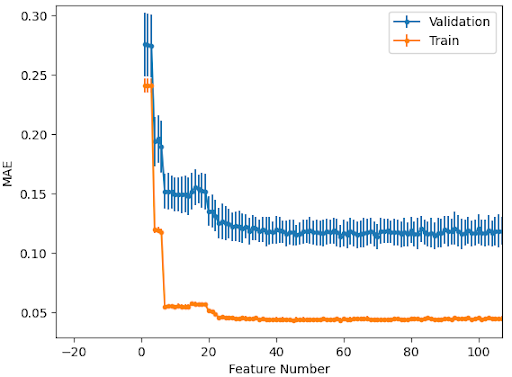
\includegraphics[width=0.95\textwidth]{figures/diffusion_learning_curve.png}
        \caption{Learning curve}
        \label{diffusion_learning_curve}
        \end{figure}
    
    \end{enumerate}
    
    \item Chemical Assessment

    \begin{enumerate}

        \item Data are aggregated and a violin plot is generated for the left out data for our $D$ score (Figure~\ref{diffusion_chemical}). We show that intuitively dissimilar materials to the Original data set, such as noble gases, are to the very right of the figure. Similar materials like transition metals are closer to the original data.

        \begin{figure}[H]
        \centering
        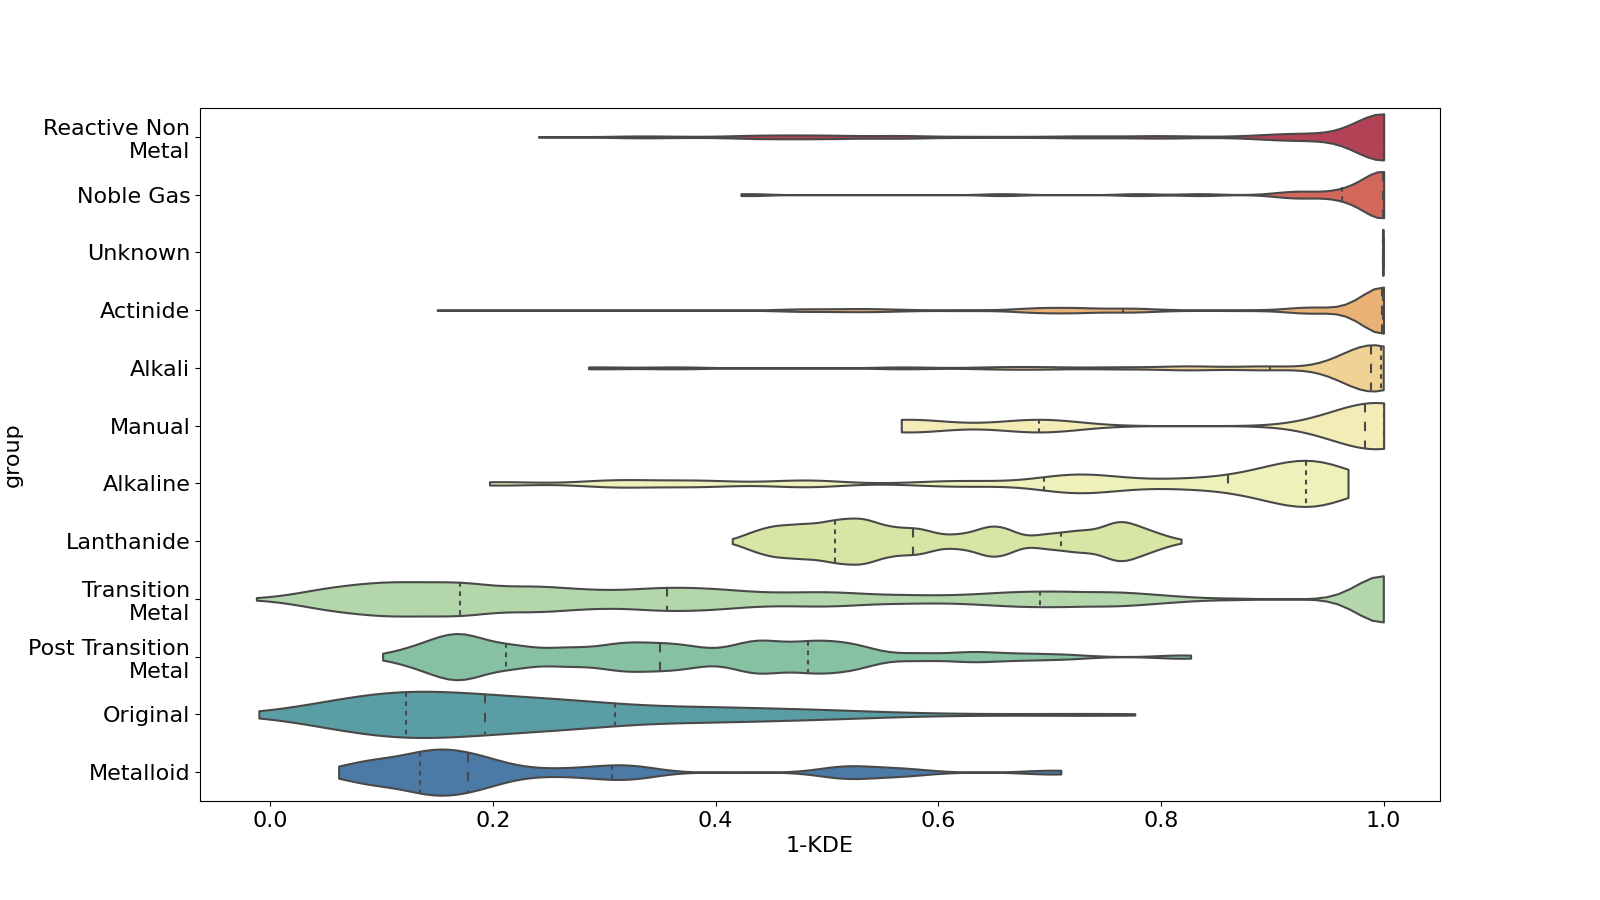
\includegraphics[width=0.95\textwidth]{figures/diffusion_chemical.png}
        \caption{Violin}
        \label{diffusion_chemical}
        \end{figure}

        \item From the domains assigned in our methods section, we acquire the PR curve shown in Figure~\ref{diffusion_chemical_pr}.

        \begin{figure}[H]
        \centering
        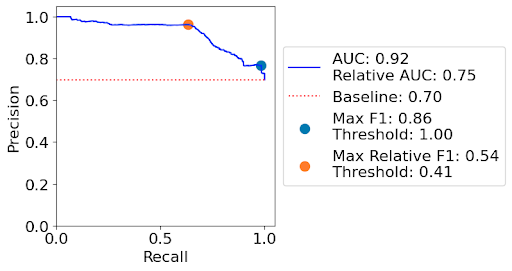
\includegraphics[width=0.95\textwidth]{figures/diffusion_chemical_pr.png}
        \caption{PR - Need to update this figure. Acts as placeholder.}
        \label{diffusion_chemical_pr}
        \end{figure}
        
    \end{enumerate}
    
    \item Numerical Single Assessment

    \begin{enumerate}

        \item Aggregated data from single numerical tests are shown in Figure~\ref{diffusion_single}. We show that our residuals grow as our $D$ score increases.

        \begin{figure}[H]
        \centering
        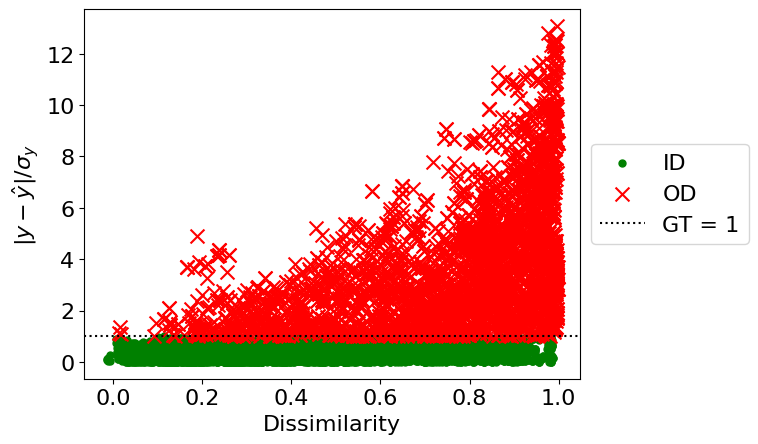
\includegraphics[width=0.95\textwidth]{figures/diffusion_single.png}
        \caption{Numerical}
        \label{diffusion_single}
        \end{figure}

        \item The associated precision recall curve is shown in Figure~\ref{diffusion_single_pr}.

        \begin{figure}[H]
        \centering
        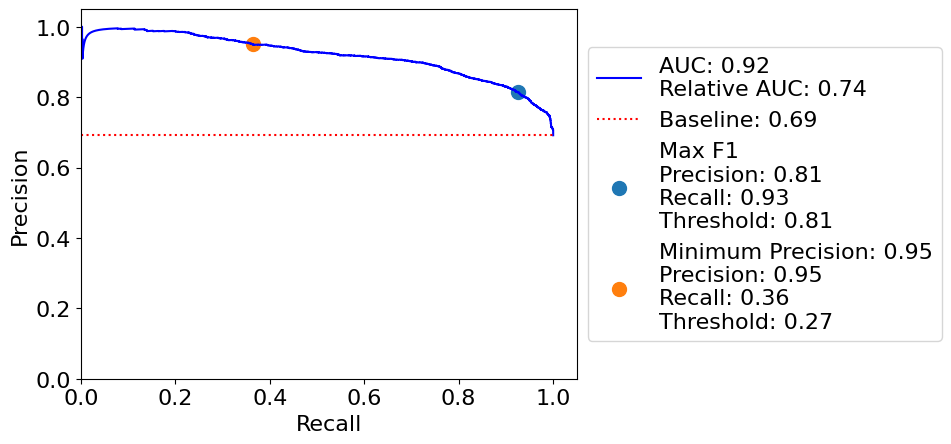
\includegraphics[width=0.95\textwidth]{figures/diffusion_single_pr.png}
        \caption{PR}
        \label{diffusion_single_pr}
        \end{figure}
    \end{enumerate}

    \item Numerical Statistical Assessment

    \begin{enumerate}
        \item We bin our data with respect to our $D$ score into 10 bins of with an equal number of points.

        \item We compare how z-score for each bin compare to a standard normal distribution (miscalibration area) and is sown in Figure~\ref{diffusion_stat}. Miscalibration area increases as data becomes increasingly dissimilar.

        \begin{figure}[H]
        \centering
        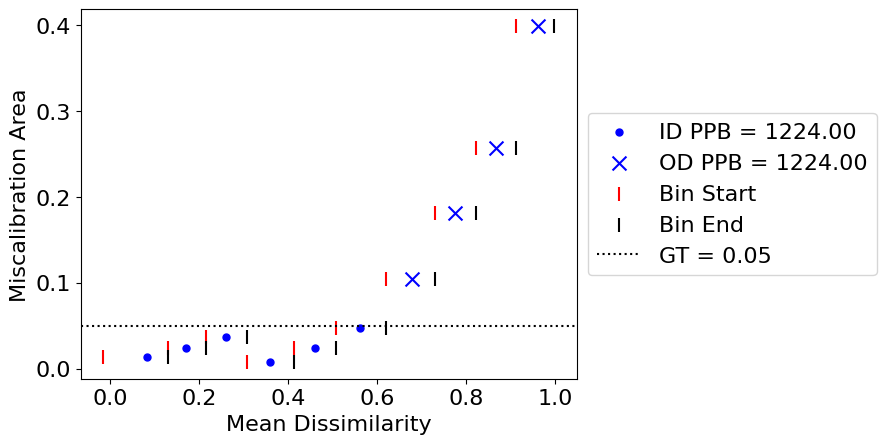
\includegraphics[width=0.95\textwidth]{figures/diffusion_stat.png}
        \caption{Numerical}
        \label{diffusion_stat}
        \end{figure}

        \item Our $D$ measure perfectly separates ID from OD data in this case in Figure~\ref{diffusion_stat_pr}.

        \begin{figure}[H]
        \centering
        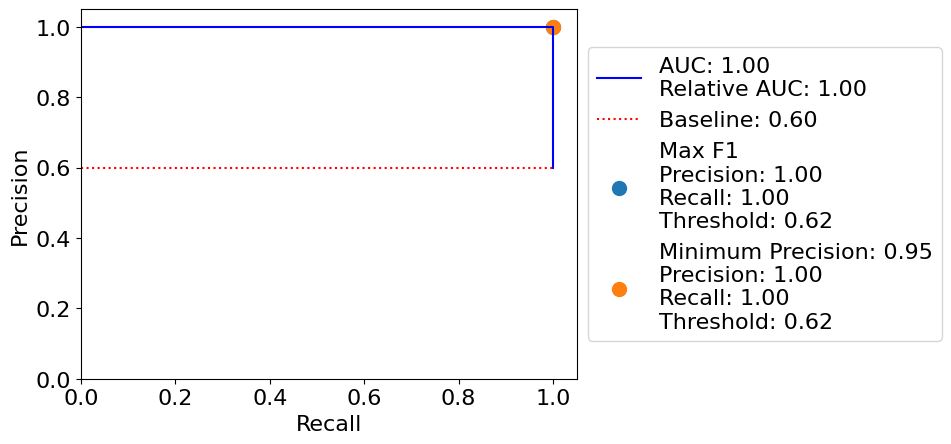
\includegraphics[width=0.95\textwidth]{figures/diffusion_stat_pr.png}
        \caption{PR}
        \label{diffusion_stat_pr}
        \end{figure}
        
    \end{enumerate}
    
\end{enumerate}

\subsection{Steel Yield Strength}

\begin{enumerate}
    \item Data Curation and Feature Selection

    \begin{enumerate}

        \item Using the original data, features were down selected from 377 to 7 features using the EnsembleModelfEatureSelector from MAST-ML. The corresponding learning curve is shown in Figure~\ref{steel_learning_curve}.


    \begin{figure}[H]
    \centering
    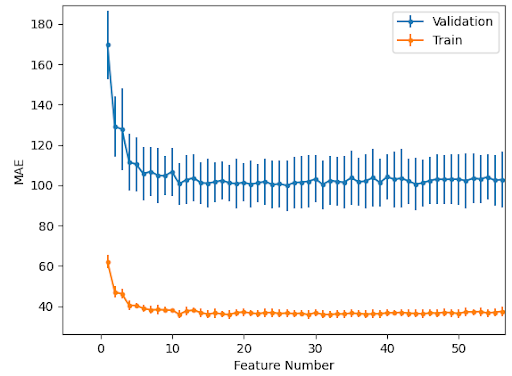
\includegraphics[width=0.95\textwidth]{figures/steel_learning_curve.png}
    \caption{Learning curve}
    \label{steel_learning_curve}
    \end{figure}
    
    \end{enumerate}
    
    \item Chemical Assessment

    \begin{enumerate}

        \item Data are aggregated and a violin plot is generated for the left out data for our $D$ score (Figure~\ref{steel_chemical}). Note that the Pertubed Original data are within the range of $D$ values and their median values align. All other data are further away from the Original data set. However, the Iron Based Far data are closer than the Copper Based and Aluminum Based sets. The observation is reasonable considering most of the Original data are iron based, but outside the range of iron weight percentages in the Original set.

        \begin{figure}[H]
        \centering
        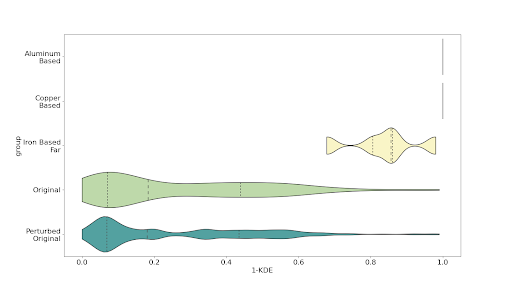
\includegraphics[width=0.95\textwidth]{figures/steel_chemical.png}
        \caption{Violin}
        \label{steel_chemical}
        \end{figure}

        \item From the domains assigned in our methods section, we acquire the PR curve shown in Figure~\ref{steel_chemical_pr}.

        \begin{figure}[H]
        \centering
        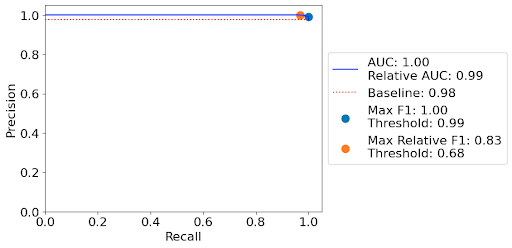
\includegraphics[width=0.95\textwidth]{figures/steel_chemical_pr.png}
        \caption{PR - Need to update this figure. Acts as placeholder.}
        \label{steel_chemical_pr}
        \end{figure}
        
    \end{enumerate}
    
    \item Numerical Single Assessment

    \begin{enumerate}

        \item Aggregated data from numerical tests are shown in Figure~\ref{steel_single}. We show that our residuals grow as our $D$ score increases.

        \begin{figure}[H]
        \centering
        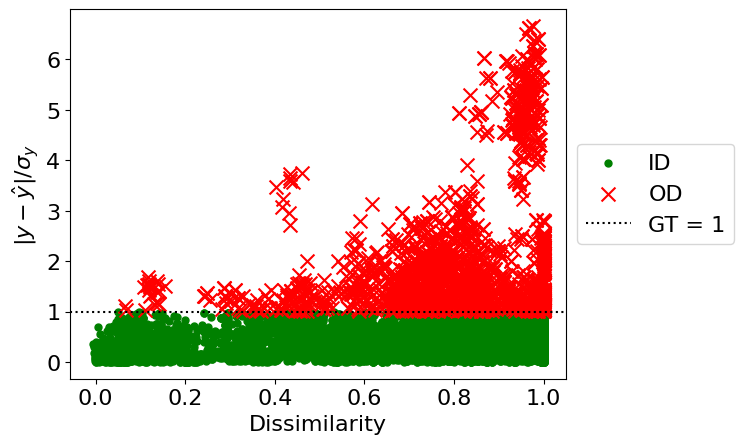
\includegraphics[width=0.95\textwidth]{figures/steel_single.png}
        \caption{Numerical}
        \label{steel_single}
        \end{figure}

        \item The associated precision recall curve is shown in Figure~\ref{steel_single_pr}.

        \begin{figure}[H]
        \centering
        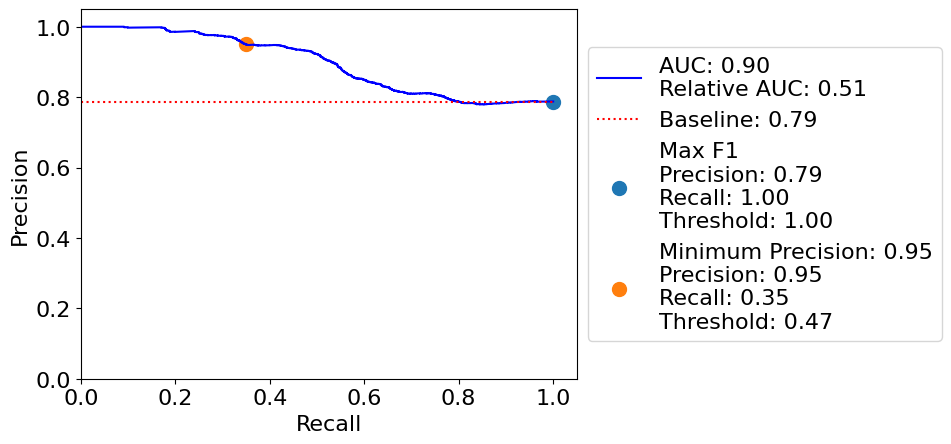
\includegraphics[width=0.95\textwidth]{figures/steel_single_pr.png}
        \caption{PR}
        \label{steel_single_pr}
        \end{figure}
    \end{enumerate}

    \item Numerical Statistical Assessment
    
    \begin{enumerate}
        \item We bin our data with respect to our $D$ score into 10 bins of with an equal number of points.

        \item We compare how z-score for each bin compare to a standard normal distribution (miscalibration area) and is sown in Figure~\ref{steel_stat}. Miscalibration area is greater to the right of around 0.5 compared to the left.

        \begin{figure}[H]
        \centering
        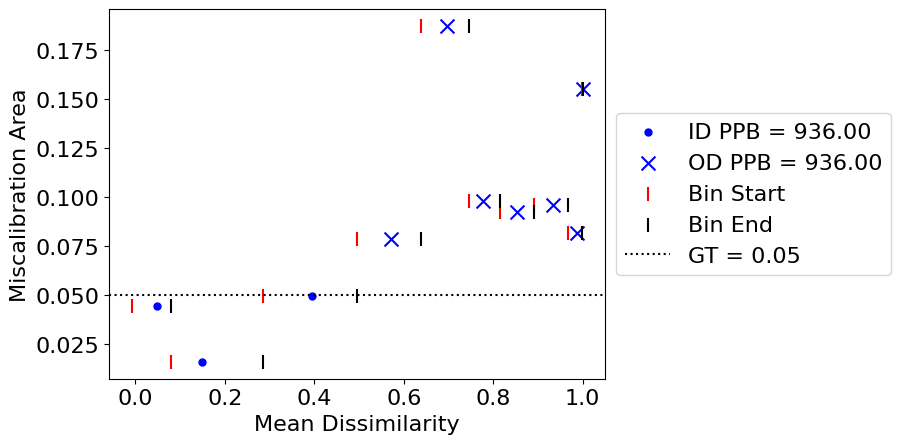
\includegraphics[width=0.95\textwidth]{figures/steel_stat.png}
        \caption{Numerical}
        \label{steel_stat}
        \end{figure}

        \item Our $D$ measure perfectly separates ID from OD data in this case in Figure~\ref{steel_stat_pr}.

        \begin{figure}[H]
        \centering
        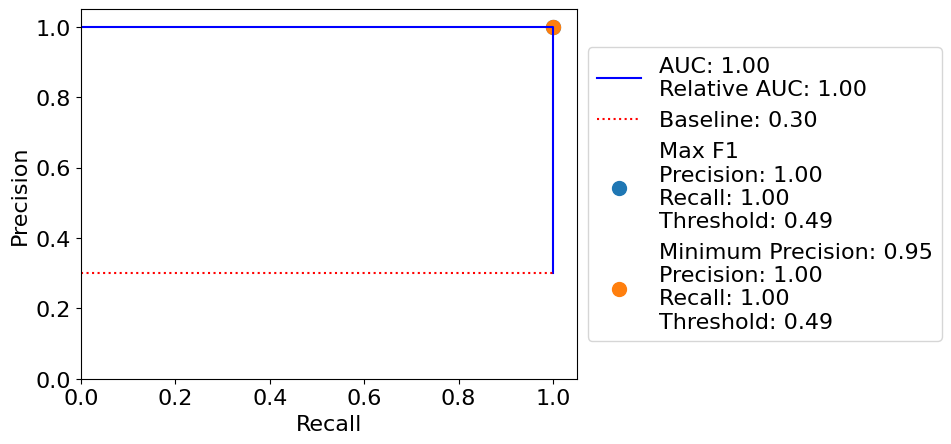
\includegraphics[width=0.95\textwidth]{figures/steel_stat_pr.png}
        \caption{PR}
        \label{steel_stat_pr}
        \end{figure}
        
    \end{enumerate}
\end{enumerate}

\subsection{Fluence}

\begin{enumerate}
    
    \item Chemical Assessment

    \begin{enumerate}

        \item Data are aggregated and a violin plot is generated for the left out data for our $D$ score (Figure~\ref{fluence_chemical}). Note that the Pertubed Original data are within the range of $D$ values and their median values align. All other data are further away from the Original data set.

        \begin{figure}[H]
        \centering
        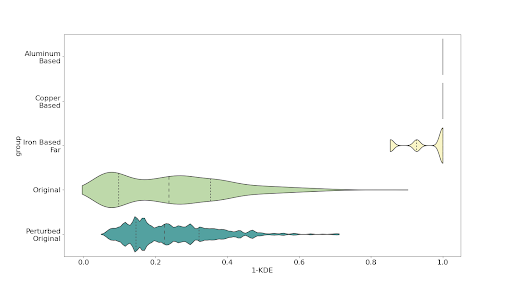
\includegraphics[width=0.95\textwidth]{figures/fluence_chemical.png}
        \caption{Violin}
        \label{fluence_chemical}
        \end{figure}

        \item From the domains assigned in our methods section, we acquire the PR curve shown in Figure~\ref{fluence_chemical_pr}.

        \begin{figure}[H]
        \centering
        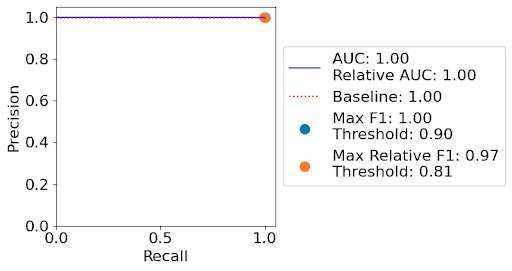
\includegraphics[width=0.95\textwidth]{figures/fluence_chemical_pr.png}
        \caption{PR - Need to update this figure. Acts as placeholder.}
        \label{fluence_chemical_pr}
        \end{figure}
        
    \end{enumerate}
    
    \item Numerical Single Assessment

    \begin{enumerate}

        \item Aggregated data from numerical tests are shown in Figure~\ref{fluence_single}. We show that our residuals grow as our $D$ score increases.

        \begin{figure}[H]
        \centering
        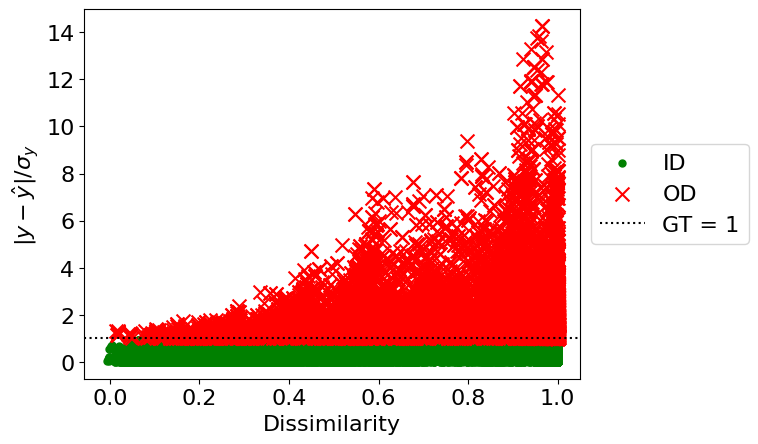
\includegraphics[width=0.95\textwidth]{figures/fluence_single.png}
        \caption{Numerical}
        \label{fluence_single}
        \end{figure}

        \item The associated precision recall curve is shown in Figure~\ref{fluence_single_pr}.

        \begin{figure}[H]
        \centering
        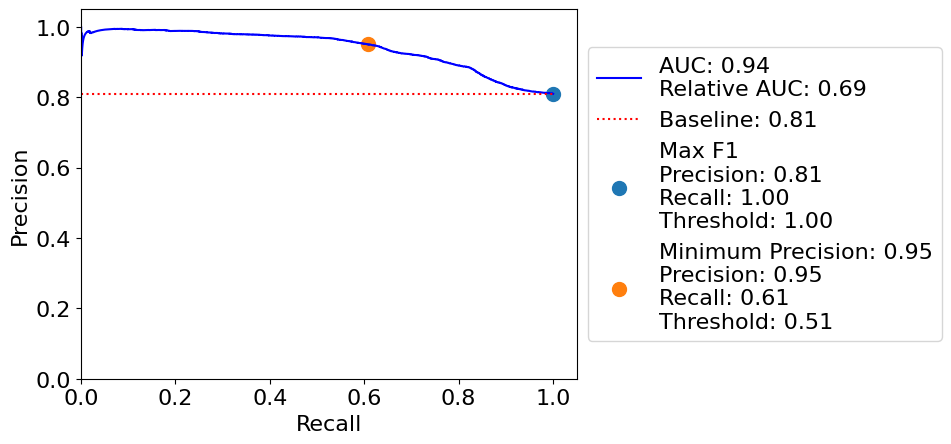
\includegraphics[width=0.95\textwidth]{figures/fluence_single_pr.png}
        \caption{PR}
        \label{fluence_single_pr}
        \end{figure}
    \end{enumerate}

    \item Numerical Statistical Assessment

    \begin{enumerate}
        \item We bin our data with respect to our $D$ score into 10 bins of with an equal number of points.

        \item We compare how z-score for each bin compare to a standard normal distribution (miscalibration area) and is sown in Figure~\ref{fluence_stat}. Miscalibration area is greater to the right of around 0.5 compared to the left.

        \begin{figure}[H]
        \centering
        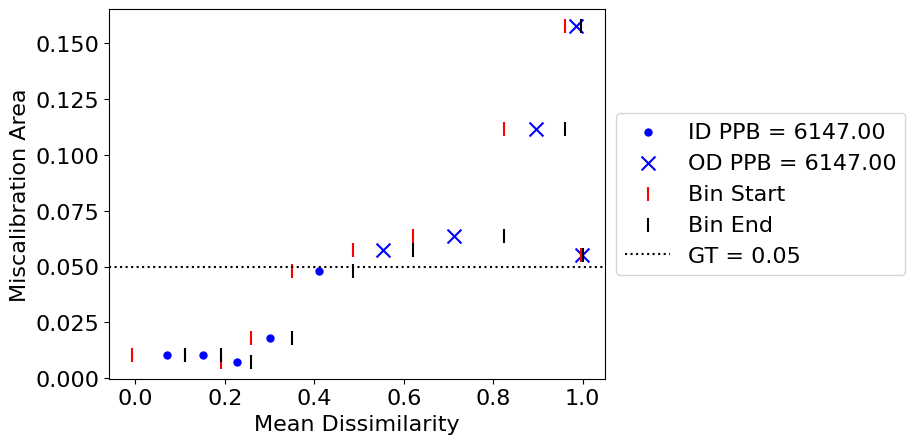
\includegraphics[width=0.95\textwidth]{figures/fluence_stat.png}
        \caption{Numerical}
        \label{fluence_stat}
        \end{figure}

        \item Our $D$ measure perfectly separates ID from OD data in this case in Figure~\ref{fluence_stat_pr}.

        \begin{figure}[H]
        \centering
        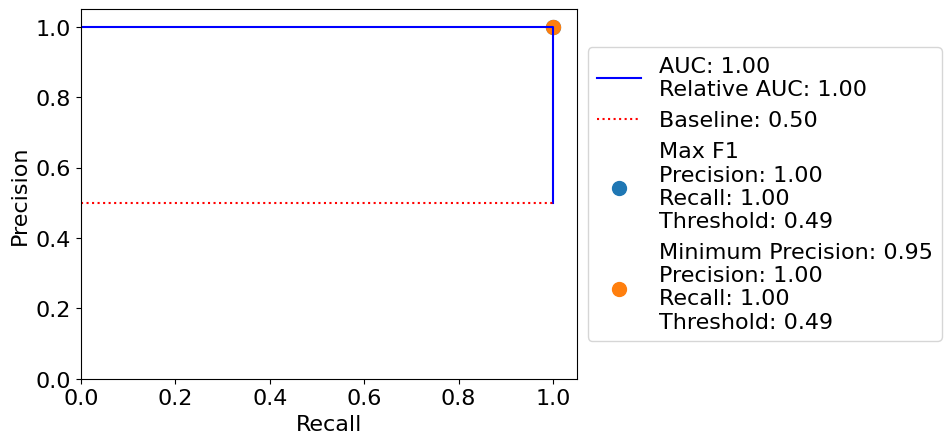
\includegraphics[width=0.95\textwidth]{figures/fluence_stat_pr.png}
        \caption{PR}
        \label{fluence_stat_pr}
        \end{figure}
        
    \end{enumerate}

\end{enumerate}

\subsection{Super Conduction}

\begin{enumerate}
    \item Chemical Assessment
    \begin{enumerate}
        \item Data are aggregated and a violin plot is generated for the left out data four our $D$ score. Figure~\ref{cond_high_chemical} has the violin plot for when we treat the majority of leave out data as $T_{low}$. As expected, our $T_{low}$ data median is near 1. 

        \begin{figure}[H]
        \centering
        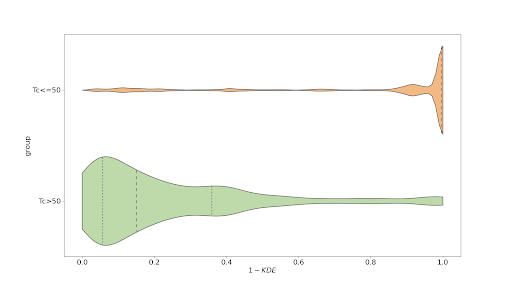
\includegraphics[width=0.95\textwidth]{figures/cond_high_chemical.png}
        \caption{Violin}
        \label{cond_high_chemical}
        \end{figure}

        \item From the domains assigned in our methods section, we acquire the PR curve shown in Figure~\ref{cond_high_chemical_pr}.

        \begin{figure}[H]
        \centering
        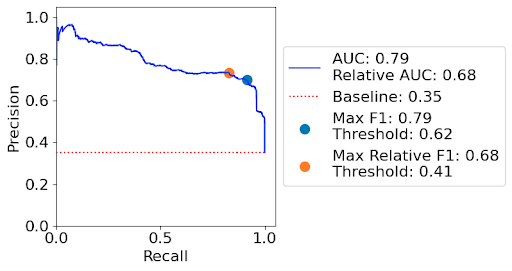
\includegraphics[width=0.95\textwidth]{figures/cond_high_chemical_pr.png}
        \caption{PR - Need to update this figure. Acts as placeholder.}
        \label{cond_high_chemical_pr}
        \end{figure}
        
        \item Figure~\ref{cond_low_chemical} has the violin plot for when we treat the majority of leave out data as $T_{high}$. Unfortunately, our $D$ measure does not show much difference in median values between $T_{low}$ and $T_{high}$. No ``good'' models can be constructed from these super conduction data. Hence, we believe our spatial measure will break down in this limit.

        \begin{figure}[H]
        \centering
        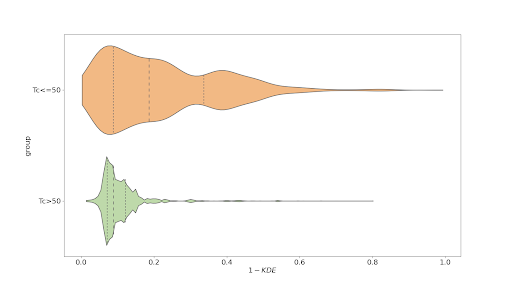
\includegraphics[width=0.95\textwidth]{figures/cond_low_chemical.png}
        \caption{Violin}
        \label{cond_low_chemical}
        \end{figure}

        \item From the domains assigned in our methods section, we acquire the PR curve shown in Figure~\ref{cond_low_chemical_pr}.

        \begin{figure}[H]
        \centering
        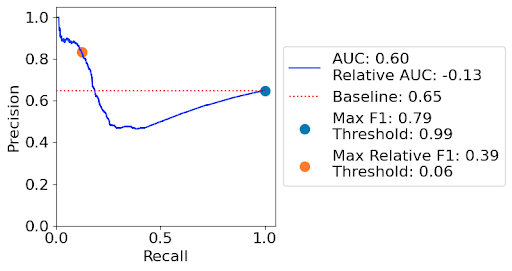
\includegraphics[width=0.95\textwidth]{figures/cond_low_chemical_pr.png}
        \caption{PR - Need to update this figure. Acts as placeholder.}
        \label{cond_low_chemical_pr}
        \end{figure}

    \end{enumerate}

    \item Numerical Single Assessment

    \begin{enumerate}

        \item Aggregated data from numerical tests are shown in Figure~\ref{cond_single}. Unusually, absolute residuals grow initially, but then decrease at $D$ is at its highest.

        \begin{figure}[H]
        \centering
        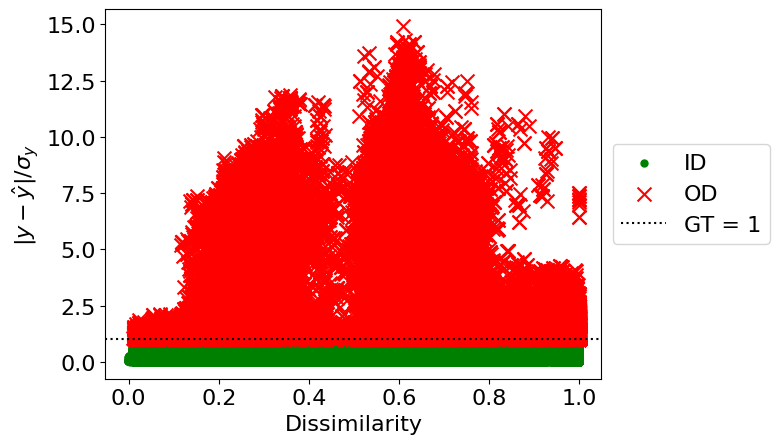
\includegraphics[width=0.95\textwidth]{figures/cond_single.png}
        \caption{Numerical}
        \label{cond_single}
        \end{figure}

        \item The associated precision recall curve is shown in Figure~\ref{cond_single_pr}.

        \begin{figure}[H]
        \centering
        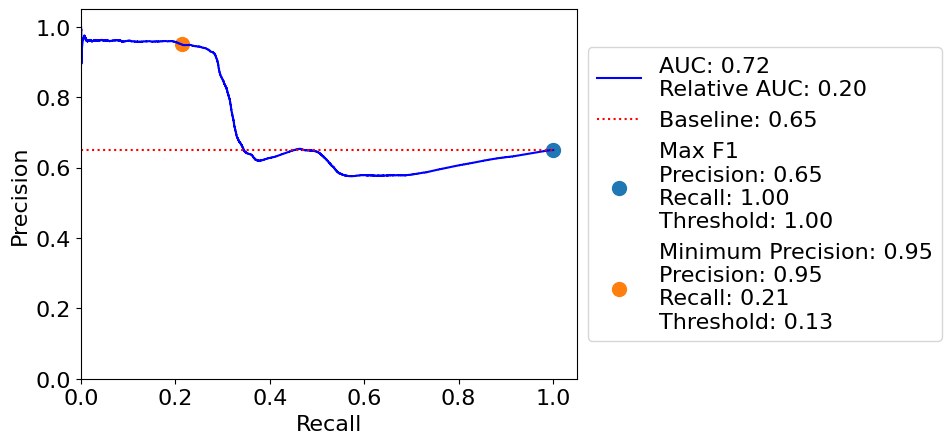
\includegraphics[width=0.95\textwidth]{figures/cond_single_pr.png}
        \caption{PR}
        \label{cond_single_pr}
        \end{figure}
    \end{enumerate}

    \item Numerical Statistical Assessment

    \begin{enumerate}
        \item We bin our data with respect to our $D$ score into 10 bins of with an equal number of points.

        \item We compare how z-score for each bin compare to a standard normal distribution (miscalibration area) and is sown in Figure~\ref{cond_stat}. Miscalibration area is greater to the right of around 0.2 compared to the left.

        \begin{figure}[H]
        \centering
        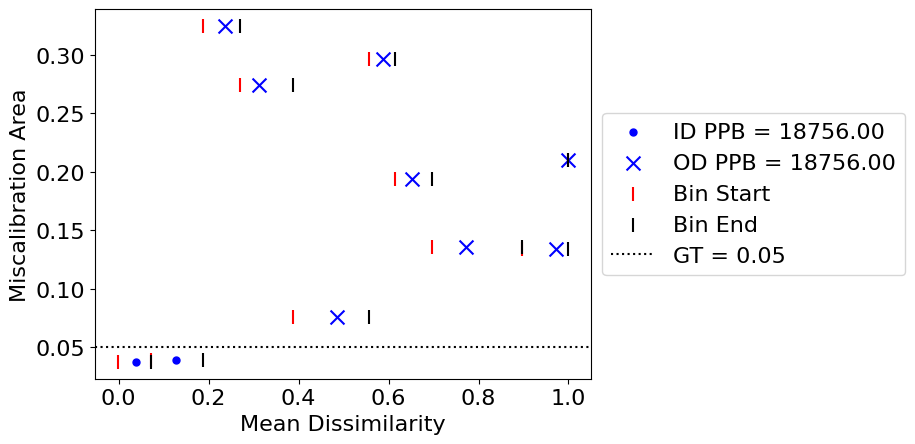
\includegraphics[width=0.95\textwidth]{figures/cond_stat.png}
        \caption{Numerical}
        \label{cond_stat}
        \end{figure}

        \item Our $D$ measure perfectly separates ID from OD data in this case in Figure~\ref{cond_stat_pr}.

        \begin{figure}[H]
        \centering
        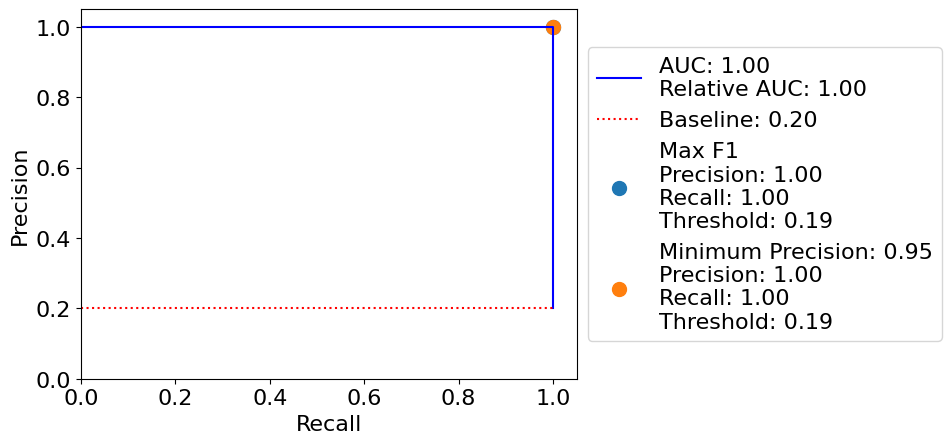
\includegraphics[width=0.95\textwidth]{figures/cond_stat_pr.png}
        \caption{PR}
        \label{cond_stat_pr}
        \end{figure}
        
    \end{enumerate}
    
\end{enumerate}

\subsection{Friedman}

\begin{enumerate}
    \item Numerical Single Assessment

    \begin{enumerate}

        \item Aggregated data from numerical tests are shown in Figure~\ref{friedman_single}.

        \begin{figure}[H]
        \centering
        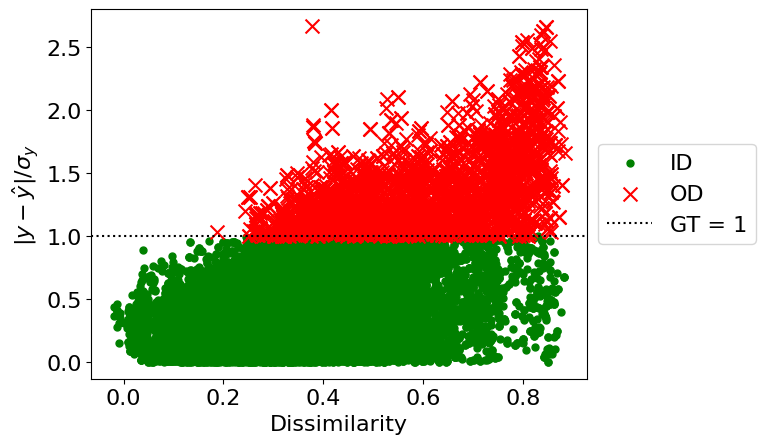
\includegraphics[width=0.95\textwidth]{figures/friedman_single.png}
        \caption{Numerical}
        \label{friedman_single}
        \end{figure}

        \item The associated precision recall curve is shown in Figure~\ref{friedman_single_pr}.

        \begin{figure}[H]
        \centering
        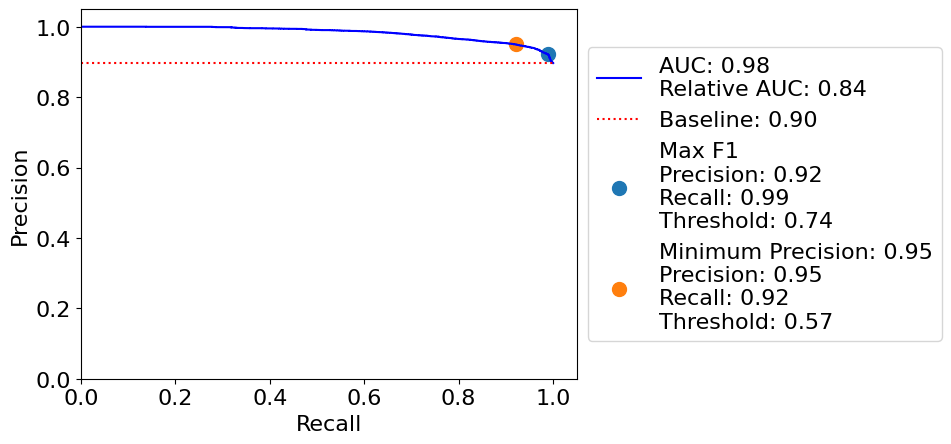
\includegraphics[width=0.95\textwidth]{figures/friedman_single_pr.png}
        \caption{PR}
        \label{friedman_single_pr}
        \end{figure}
    \end{enumerate}

    \item Numerical Statistical Assessment
    
    \begin{enumerate}
        \item We bin our data with respect to our $D$ score into 10 bins of with an equal number of points.

        \item We compare how z-score for each bin compare to a standard normal distribution (miscalibration area) and is sown in Figure~\ref{friedman_stat}. Miscalibration area First decreases until around 0.19 and then being to increase after around 0.29. 

        \begin{figure}[H]
        \centering
        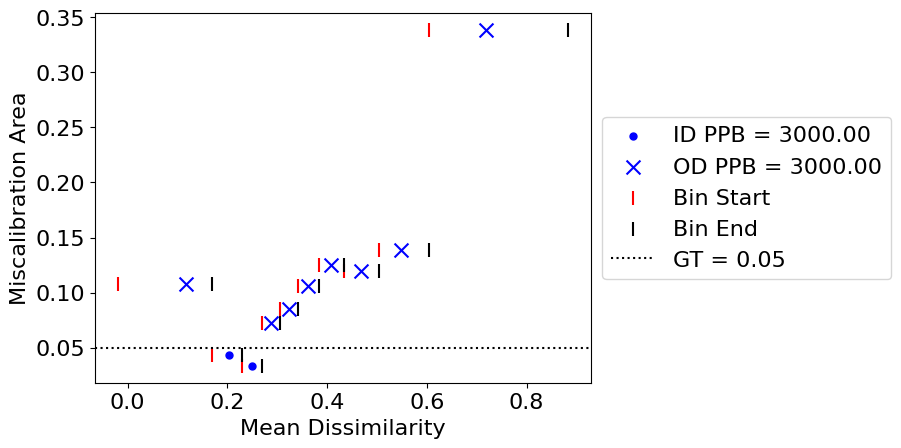
\includegraphics[width=0.95\textwidth]{figures/friedman_stat.png}
        \caption{Numerical}
        \label{friedman_stat}
        \end{figure}

        \item Unlike all of our previous tests, our $D$ measure does not perfectly separates ID from OD data Figure~\ref{friedman_stat_pr}. Unusually, our closest interval of points are miscalibrated.

        \begin{figure}[H]
        \centering
        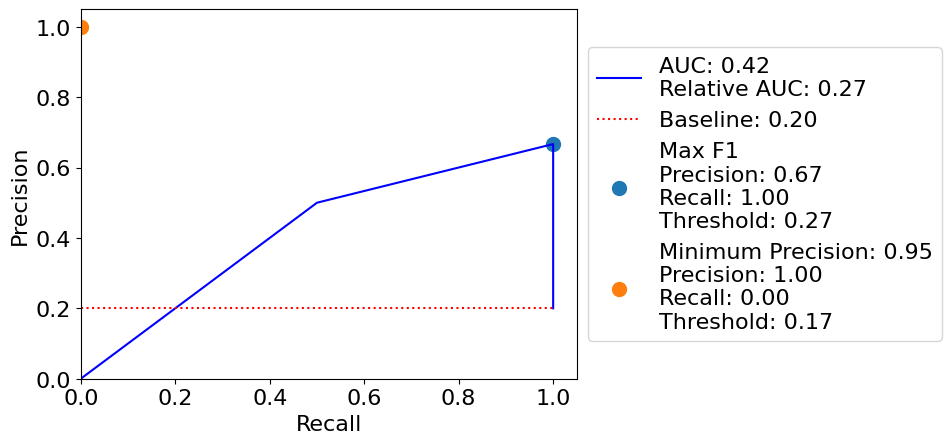
\includegraphics[width=0.95\textwidth]{figures/friedman_stat_pr.png}
        \caption{PR}
        \label{friedman_stat_pr}
        \end{figure}
        
    \end{enumerate}

\subsection{Aggregate Results}

\begin{enumerate}
    \item Include all major results in a table similar to that in Table~\ref{aggregate_results}.
    \item We note that for the vast majority of tests and data sets, our $D$ is a success.
\end{enumerate}

\begin{table}[H]
\begin{tabular}{|l|l|l|l|l|l|}
\hline
\textbf{Data} & \textbf{Domain}       & \textbf{Baseline} & \textbf{AUC} & \textbf{Relative AUC} & \textbf{Max F1} \\ \hline
diffusion     & chemical              &                   &              &                       &                 \\ \hline
diffusion     & single numerical      &                   &              &                       &                 \\ \hline
diffusion     & statistical numerical &                   &              &                       &                 \\ \hline
...           &                       &                   &              &                       &                 \\ \hline
\end{tabular}
\caption{All results}
\label{aggregate_results}
\end{table}

\end{enumerate}
\section{Conclusion}

\begin{enumerate}
    \item We have shown that our $D$ score scales with chemical intuition for what should be ID or OD.
    \item We have shown that our $D$ scores do scale with residuals on average, and give us information for discerning higher and lower uncertainties via our precision recall curves.
    \item The $D$ score can also measure how dissimilar data can become before z-scores are no longer distributed in a standard normal way.
    \item Our $D$ score is powerful because it learns from the feature space alone could be added to many model types.
    \item Both the single and statistical numerical methods are easily implementable thorugh the MAST-ML package (or at least will be).
\end{enumerate}
\section{Data Availability}

\begin{itemize}
    \item Figsharevim-latexsuite
    \item GitHub
\end{itemize}

\par
The raw and processed data required to reproduce these findings are available to download from figshare at \url{https://figshare.com/} and GitHub at \url{https://github.com/}.
\section{Acknowledgements}

\par
Lane E. Schultz is grateful for the Bridge to the Doctorate: Wisconsin Louis Stokes Alliance for Minority Participation National Science Foundation (NSF) award number HRD-1612530, the University of Wisconsin– Madison Graduate Engineering Research Scholars (GERS) fellowship program for the financial support for graduate student investigation, and the PPG Coating Innovation Center for financial support. Other authors gratefully acknowledge support from the NSF Collaborative Research: Framework: Machine Learning Materials Innovation Infrastructure award number 1931306. Machine learning was performed with the computational resources provided by the Extreme Science and Engineering Discovery Environment (XSEDE), National Science Foundation Grant No. OCI-1053575.

\pagebreak
\printbibliography[heading=bibintoc]
\pagebreak
\section{Supplemental}

\subsection{Cram\'er-von Mises Test}

\par Hypothesis testing can be used as an intuitive statistical ground truth for our binned z-scores. Any two distributions can be compared using the Cram\'er-von Mises Test and do not have to be parametric. The null hypothesis is that our z-scores follow a standard normal distribution. Our alternate hypothesis is that our z-scores do not follow a standard normal distribution. If we a p-value of 0.01 for statistical significance, then we reject our null hypothesis. We define OD as the bins where the null hypothesis is rejected and ID otherwise. As we can see from our diffusion data in Figure~\ref{p_values_small}, most data to the left of 0.6 is ID and OD beyond. Our corresponding miscalibration area is shown in Figure~\ref{area_small}.

\begin{figure}[H]
\centering
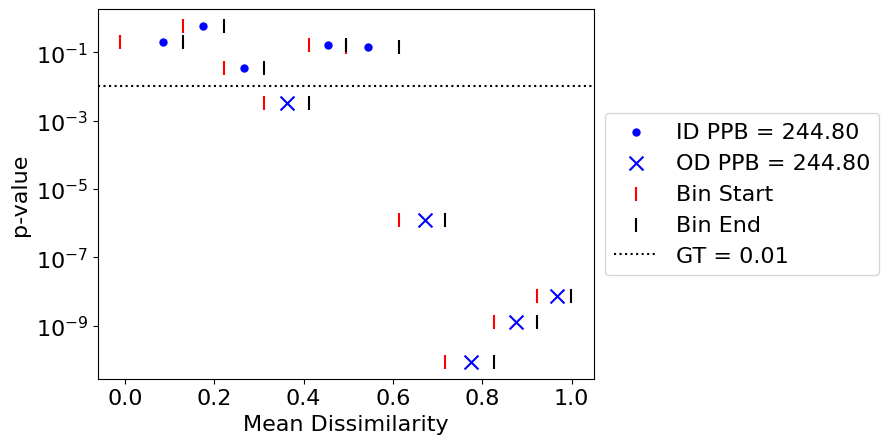
\includegraphics[width=0.95\textwidth]{figures/p_values_small.png}
\caption{PR}
\label{p_values_small}
\end{figure}

\begin{figure}[H]
\centering
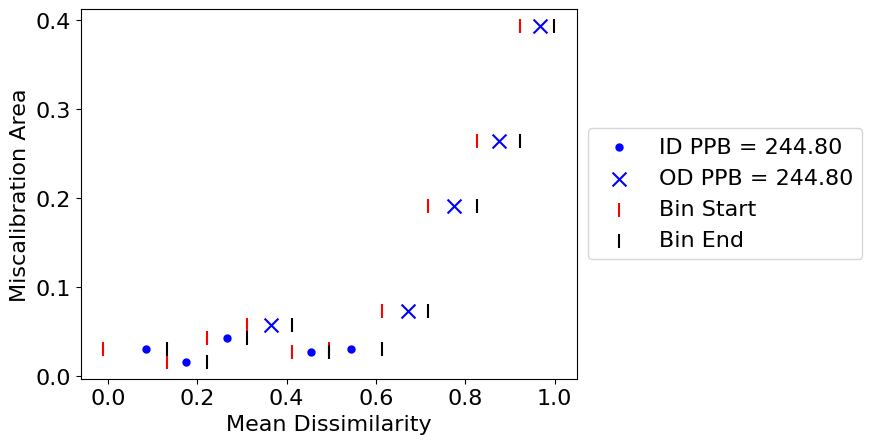
\includegraphics[width=0.95\textwidth]{figures/area_small.png}
\caption{PR}
\label{area_small}
\end{figure}

\par We can increase the number of points per bin and apply Cram\'er-von Mises Test again. We increased the number of points per bin from 244.80 to 1101.60. The p-values are shown in Figure~\ref{p_values_large} and their corresponding miscalibration area are shown in Figure~\ref{area_large}. Although miscalibration areas between Figures~\ref{area_small} and \ref{area_large} do not significantly differ, our p-values from Figures~\ref{p_values_small} and \ref{p_values_large} do change significantly for the second and third bins from the left. This can be attributed to the dependent sampling from our repeated CV. Our methodology of repeatedly splitting our data with K-fold CV and our leave one cluster our CV makes our sampling increasingly dependent.

\begin{figure}[H]
\centering
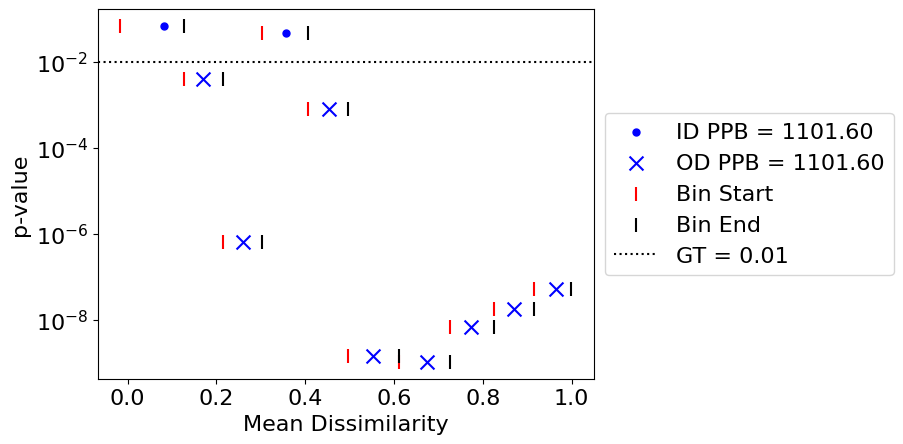
\includegraphics[width=0.95\textwidth]{figures/p_values_large.png}
\caption{PR}
\label{p_values_large}
\end{figure}

\begin{figure}[H]
\centering
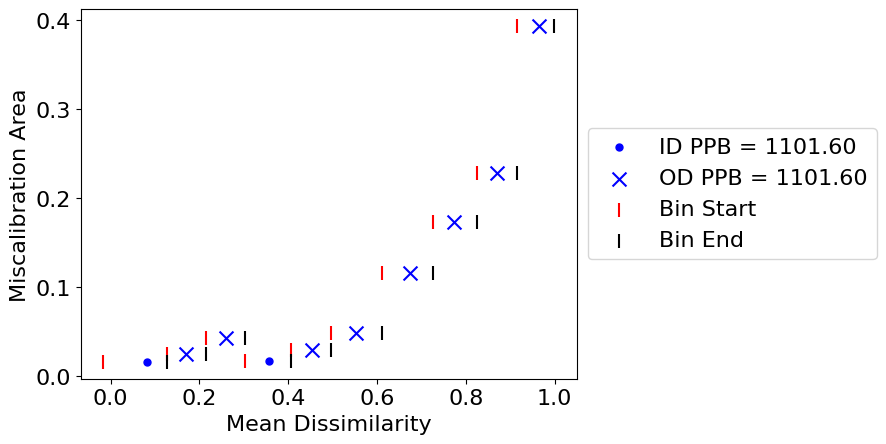
\includegraphics[width=0.95\textwidth]{figures/area_large.png}
\caption{PR}
\label{area_large}
\end{figure}

\end{document}
